\section{Background}
\label{sec:background}

\begin{figure}
	\centering
	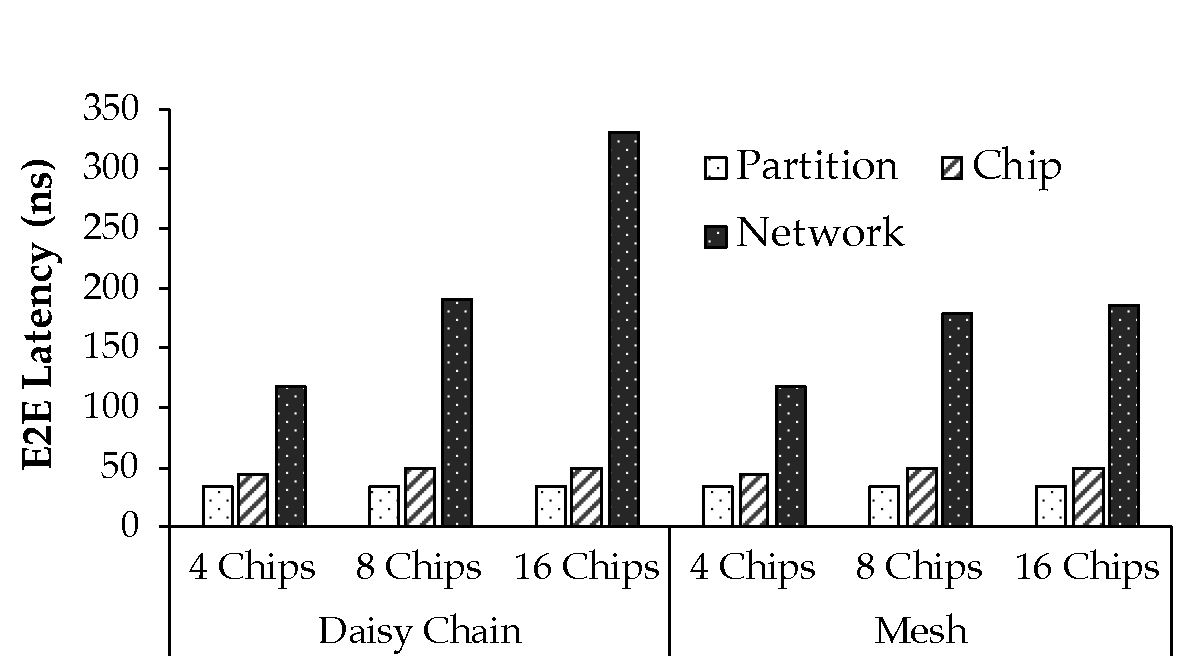
\includegraphics[width=.85\columnwidth]{graphs/e2elatency-pattern.pdf}
	\caption{End-to-end latency of memory accesses.}
	\label{fig:e2elat}
\end{figure}


%\subsection{3D Memories}

\javier{Points to come across:

\begin{itemize}
  \item SW trend: Servers workloads are keeping their datasets memory resident; HW trend: Due to slowdown in silicon density and efficiency, computer system are integrating custom logic (accelerators).
  \item Explain the programmability benefits of pointer-is-a-pointer AND flexible VM system (e.g., demand paging, COW) of a conventional translation mechanism.
  \item TLB Reach Problem: Explain that a conventional translation mechanism is not effective for accelerators because (1) it relies on deep cache and TLB hierarchies and (2) data reuse, to bridge the gap between computation speed and memory capacity. However, accelerators primarily exploit parallel access with proximity to memory, and not reuse and deep cache hierarchies. Furthermore, accelerator are custom and hence silicon optimized, hence the available budget for translation hardware is limited. I think we can just cite prior work on TLB miss rates for in-memory workloads.   
  \item TLB Penalty Problem: Explain that compute and memory are scaling-out due to the slowdown in silicon scaling and efficiency, hence TLB misses (page walks) become more costly. We can show something similar to Figure 1 here.
\end{itemize}


}

%3D memory enables vertical stacks of multiple DRAM dies on top of a logic layer within a single package, leveraging low-latency/high-bandwidth through-silicon vias (TSVs). Two well-known incarnations of 3D memory technology are Micron's Hybrid Memory Cube (HMC)~\cite{hmc} and JEDEC's High Bandwidth Memory (HBM)~\cite{jedec:high}. Fig.~\ref{fig:overview}a illustrates the anatomy of a 3D memory chip. The chip consists of multiple vertical memory partitions, called vaults. Each vault is independent and similar to a conventional DDR channel, with its own DRAM controller and signals. Each DRAM controller connects to all the DRAM dies through a TSV bus. Similar to previous studies, MPUs are scattered across the vaults~\cite{ahn:scalable, gao:practical, pugsley:ndc, kim:neurocube}, while a network-on-chip (NoC) connects the vaults to each other and to the off-package links.

%Architectures that deploy 3D memories consist of a pool of CPUs and memory chips. Fig.s~\ref{fig:overview}b,~\ref{fig:overview}c,~and~\ref{fig:overview}d show the memory organizations considered in this paper. The CPU is connected to multiple memory chips using high-speed point-to-point SerDes links and a packet-based communication protocol. Fig.~\ref{fig:overview}b depicts a star topology where the CPU is connected to a small number of memory chips~\cite{fujitsu:while, reinders:knights}. Larger memory systems interconnect dozens of chips in a daisy chain (Fig.~\ref{fig:overview}c), which minimizes the number of links~\cite{gao:practical, pugsley:ndc}, or a mesh (Fig.~\ref{fig:overview}d), which minimizes the number of hops~\cite{ahn:scalable, kim:memory-centric}. 

%Memory accesses within the local partition are much cheaper than accesses to remote partitions, as the latter involves traversing expensive NoC and/or cross-chip interconnects. Fig.~\ref{fig:e2elat} compares the average end-to-end memory access latency depending on the target data's location: 1) same partition, 2) different partition, same chip, and 3) any chip in the network. The three cases are labeled as \textit{Partition}, \textit{Chip}, and \textit{Network} respectively. Unsurprisingly, the location of the data significantly affects latency. A data access in the local partition is the fastest; accessing a remote partition within the same chip is around $1.4\times$ slower, while accessing remote memory chips increases the latency by $3.5$--$10\times$, depending on the network and memory chip count. In summary, %these results indicate that optimizing for memory access latency requires MPUs to localize memory accesses within their partitions.

%\subsection{Unified Virtual Memory}
%\label{sec:uvm}

No prior proposal for virtually addressed MPUs is both general and efficient. The simplest approaches offload the address translation task to the CPU cores or an IOMMU~\cite{oskin:active, vesely:observation, gao:practical, xi:beyond}. Though simple, the fact that the MPUs and CPUs are on different chips means that sending translation requests to the CPU results in expensive chip-to-chip communication. Alternatively, one can integrate a traditional MMU with a TLB hierarchy per MPU. However, due to the limited reach of modern TLBs, page walks occur frequently, resulting in costly cross-chip traffic, as the multiple levels of the page table~\cite{gantz:hybrid} are arbitrarily scattered across the memory chips. All of these existing techniques create excessive cross-chip traffic, either to reach the CPU or to perform page walks, which could account for latencies of hundreds of nanoseconds, dramatically increasing the translation overhead.

Several recent proposals seek to improve the TLB reach. The most common approach is the introduction of larger page sizes~\cite{transparenthugepages, lighugetlbfs}. Similarly, CoLT~\cite{pham:colt} and Clustered TLBs~\cite{pham:increasing} coalesce 4-8 page translations into a single TLB entry, as long as their physical locations are contiguously in memory. Although the TLB reach improves, it is still unable to cover the entirety of a large memory system with tens or hundreds of GBs~\cite{gandhi:range}. More innovative ways of improving TLB coverage employ variable-size segments instead of fixed page-based translations~\cite{karakostas:redundant, park:hybrid, basu:efficient}. Unfortunately, the effectiveness of these techniques relies on the OS to allocate contiguous chunks of physical memory, which is not possible when the system is under memory pressure. Hence, page walks are still common in some scenarios, accounting for translation overheads of hundreds of nanoseconds. 

To summarize, there is no single approach capable of providing a unified VM that is suitable for all use cases. Prior work attempts to exploit contiguity in the physical memory, which is not always available. In contrast, our study focuses on sidestepping the need for fewer TLB misses by overlapping them with data fetch.






